\documentclass{article}
\usepackage[T1]{fontenc}

\usepackage[french]{babel}
\usepackage{parskip}
\usepackage[margin=4cm]{geometry}
\usepackage{graphicx}

\title{Rapport projet PFA}
\author{Erwan LEMATTRE \and Ewen DUFOUR}
\date{Avril 2024}

\begin{document}
\maketitle

\newpage

\section{Le jeu}
Le jeu \textit{Arthur la quête de la cuillère} a pour but d'offrir aux joueurs une expérience 
de jeu agréable avec différents niveaux ayant chacun sa spécificité tout en racontant une histoire.
L'histoire est le fil conducteur du jeu: elle permet de donner un sens aux différents niveaux.

\textit{Arthur la quête de la cuillère} s'inspire en partie de la légende du roi Arthur et
 de la série \textit{Kaamelott}. Nous avons essayé d'ajouter des références à la série tout 
en gardant un jeu cohérent pour les non-connaisseurs. On retrouve également une référence 
à \textit{Star Wars} avec les opening des niveaux inspirés de ceux des films. Enfin, 
le joueur est accompagné d'une série de musiques médiévales tout au long du jeu qui le 
plonge d'avantage dans l'aventure du roi arthur.

Le jeu se compose de 4 niveaux et d'un menu. Le \textbf{menu} sert uniquement d'accueil du jeu.
Le \textbf{niveau 1} introduit la problématique de l'histoire (opening) et permet au joueur de 
prendre en main le jeu avec un niveau plutôt simple. Le \textbf{niveau 2} lance réellement la 
quête du roi. Le joueur ayant une maîtrise des commandes du jeu, il doit maintenant parcourir un 
niveau plus difficile. On reste dans le même environnement plutôt plaisant. Avec le \textbf{niveau 3} 
les choses se compliquent. L'environnement devient plus hostile et la difficulté augmente. Le sol 
est maintenant glissant, les blocs sont plus espacés, certains blocs sont invisibles et les ennemis sont 
plus nombreux. Enfin le \textbf{niveau 4} est le niveau final dans lequel le joueur doit faire face 
au boss final. L'environnement devient lugubre, la musique indique au joueur la bataille finale.
Une fois le squelette éliminé la quête est terminée, on retourne au menu.

Il existe 3 ennemis différents dans notre jeu. Les archers (niveaux 1, 2 et 3), les chevaliers (niveaux 1, 2 et 3)
et \textbf{Alexandre Le Petit} l'ennemi final (niveau 4). Les \textbf{archers} ne se déplacent pas, ils tirent des 
flèches lorsque le joueur leur fait face. Les \textbf{chevaliers} suivent le joueur pour l'attaquer avec leurs 
épées. L'ennemi final peut tirer des boules de feu et mettre des coups d'épée. Ils suit également le joueur.

Le joueur de son côté a différentes capacités qui s'ajoutent à mesure que les niveaux augmentent. Au niveau 1 le 
joueur n'a aucune capacité particulière il peut seulement se déplacer et mettre des \textbf{coups d'épée}. Au niveau 2 
le joueur peut utiliser la \textbf{téléportation} qui lui permet de se déplacer très rapidement en un coup. 
Attention la téléportation ne permet cependant pas de passer au travers des objets de l'environnement ou des 
ennemis. Au niveau 3 s'ajoute les \textbf{boules de feu} qui est l'attaque à distance du joueur. Au niveau 4 le 
joueur a les mêmes capacités qu'au niveau 3. Enfin le joueur peut trouver des \textbf{soins} dans les niveaux. 
Les soins sont représentés par les items poulet.

Nous avons pu mentionner précédemment que chaque niveau possède une musique 
différente afin de varier l'ambience. Nous avons voulu faire en sorte que plus le joueur avance dans le jeu,
 plus la musique devient pesante.

Pour terminer, le jeu se joue avec les touches \verb|zqd| (ou directionnelles) pour les déplacements. Les 
touches utiles aux pouvoirs dépendent des préférences des joueurs. On utilise par défaut \verb|Shift|, 
\verb|space| et \verb|s|. D'autres touches servent au débogage, nous le verrons dans une section dédiée. 
Les niveaux ont été conçus de manière à ce que le joueur se serve au moins une fois de chaque pouvoir 
mis à sa disposition.

\section{Organisation du code}

\subsection{Les systèmes}

L'organisation générale du jeu est proche de celle du code modèle utilisé au début de ce projet.
On retrouve dans \verb|src/systems/| l'ensemble des systèmes du jeu. Le système \textbf{control} permet 
d'avoir accès aux entrées du joueur. Il est utilisé par l'entité player et les boutons du jeu. Ce 
système va appeler une fonction dans l'entité qui va ensuite gérer les actions en fonction des entrées.
Le système \textbf{real\_time} permet de gérer les actions qui doivent se passer sans latence pour le joueur.
À chaque frame il appelle une fonction spécifique à chaque entité présente dans le système. Il permet par exemple
de gérer les ennemis. Le système \textbf{music} s'occupe de la gestion des musiques du jeu. Il contient une 
variable \verb|current_track| qui permet de sélectionner la track à jouer. Les track sont prédéfinies dans le code 
elles ne peuvent pas être modifiées depuis l'extérieur. Le système \textbf{view} permet de gérer la caméra. Nous 
reviendrons sur cette partie plus en profondeur dans la suite de ce rapport.

\subsection{Le répertoire \texttt{src}}
Le répertoire \verb|src/| contient trois nouveaux fichiers. 

Le fichier \verb|level_loader.ml| permet le chargement 
les niveaux depuis des fichiers texte. C'est une partie qui a été particulièrement intéressante à implémenter. 
L'objectif a été de pouvoir créer des niveaux sans avoir besoin de connaître le fonctionnement interne du jeu. 
Nous pensons être plutôt proche de cet objectif même si certaines choses pourraient être améliorée. Les fichiers
 textes doivent contenir un ensemble de lignes 
chacune permettant la création d'un élément du jeu. On utilise la notation \texttt{id:XxY|WxH|param} avec id 
l'identifiant de l'entité (Les identifiants des entités et leur description sont disponibles dans le fichier
 \texttt{map.md}.), XxY la position XY, WxH la largeur et hauteur de l'entité et param les paramètres 
associés à l'entité. Cette ligne est découpée pour récupérer chacune des parties. Les paramètres entrés sont 
ajoutés dans une table de hachage. Lors de la création d'une entité on récupère un type énuméré \verb|setting|
définit dans \verb|const.ml|. Ce type contient les différents paramètres possibles. Les entités peuvent ensuite
récupérer les paramètres dont elles ont besoin dans cette structure. Ce fonctionnement permet d'avoir une 
flexibilité dans les déinitions de niveau. On peut par exemple donner des paramètres qui n'existent pas, cela 
n'aura aucune influence. On peut également ne pas définir un paramètre qui est nécessaire et dans ce cas une 
valeur par défaut sera donnée sans causer d'erreur. 

Le fichier \verb|resources.ml| gère le chargement des fichiers image, texte, audio et police du jeu. Le chargement 
est effectué dans le fichier \verb|game.ml| avant d'afficher le menu au démarrage du jeu.

Le fichier \verb|config.ml| contient la définition des touches pour Javascript et Sdl. La configuration est utilisée 
par les entités utilisant le système contrôle afin d'avoir accès au nom des touches.

\subsection{Le répertoire \texttt{core}}
Le répertoire \verb|src/core/| contient 2 nouveaux fichiers.

Le fichier \verb|const.ml| contient l'ensemble des constantes du jeu. On y trouve par exemple la vitesse du joueur,
la taille des blocs, etc\dots Ce regroupement permet de modifier facilement les valeurs importantes du jeu sans 
avoir besoin de chercher tous les endroits où elles sont utilisées. Ce fichier contient également le type \verb|setting| 
dont nous avons parlé dans la section précédente.

Le fichier \verb|state.ml| contient la définition du type \texttt{state}. Ce type est utilisé par le joueur et les ennemis 
afin de contrôler les animations des attaques. L'état $0$ de state signifie qu'aucune attaque est en cours. L'état $1$ 
signifie que l'attaque est en cours. Elle est mise à jour grâce à une fonction \verb|update| qui gère l'animation en 
fonction du numéro de la frame courante.

Dans le fichier \verb|global.ml| nous avons ajouté la caméra et le joueur. On peut ainsi accéder au joueur depuis tous les 
fichiers, ce qui est utile pour gérer le comportement des ennemis.

\subsection{Components}
De nombreux composants ont été créés pour notre jeu. Les composants avec box dans leur nom permettent de créer des 
variations de box avec des comportement différents. Par exemple les \textit{hide\_box} sont des box qui sont 
ajoutés dans les systèmes \textit{draw} et \textit{view} seulement lorsque la box est en collision avec le joueur.
Ci-dessous une rapide description des composants de notre jeu.
\begin{center}
    \begin{tabular}[h]{ |c|p{10cm}| }
        \hline
        \textbf{Composant} & \textbf{Description} \\
        \hline
        alexandre & Boss final du jeu \textit{Alexandre Le Petit}. \\
        \hline
        arch & Archer, tire ne se déplace pas, tire des flèches. \\
        \hline
        arrow & Flèche tirée par l'archer. Détruite lorsqu'elle entre en collision avec n'importe quel objet. \\
        \hline
        audio & Composant audio contenant la piste d'écoute courante et le numéro de la musque écouté dans la 
        piste. \\
        \hline
        background & Utilisé pour créer le fond du menu. \\
        \hline
        box & Une box simple avec toutes les paramètres possibles dessus. \\
        \hline
        bullet & Boule de feu pour le joueur et l'ennemi final. Fonctionnement similaire à \verb|arrow|. \\
        \hline
        button & Bouton, notamment utilisé dans le menu. \\
        \hline
        camera & Composant caméra contenant le focus (discuté dans la suite). \\
        \hline
        decor & Affiche une texture tout en ayant aucune intéraction avec les autres éléments du jeu. \\
        \hline
        exit\_box & Box permettant de changer de niveau lorsque le joueur entre en collision avec. \\
        \hline
        fall\_box & Box qui est affectée par la gravité lorsque le joueur entre en collision avec. \\
        \hline
        hide\_box & Box qui est affichée seulement lorsque le joueur entre en collision avec. \\
        \hline
        hitbox & Outil de débogage, voir section tests. \\
        \hline
        hpbar & Barre affichant la vie de l'ennemi final. Affiche un rectangle proportionnel à la vie du composant \verb|alexandre|. \\
        \hline
        jump\_box & Box permettant de faire rebondir le joueur. Le fait de pouvoir rebondir plus haut implique une élasticité 
        supérieure à 1. Or une élasticité supérieure à 1 fait rebondir de plus en plus haut le joueur. C'est pourquoi on à limité la 
        vélocité dans le système \textit{collisions} en utilisant \verb|clamp| du module \verb|Vector| (ajouté). \\
        \hline
        knight & Chevalier, attaque seulement avec une épée et suit le joueur lorsqu'il est assez près. \\
        \hline
        medkit & Soin pour le joueur. \\
        \hline
        opening & Opening en début de niveau. Crée le texte de l'opening et gère la caméra. Une fois l'opening terminé 
        le texte est retiré des systèmes et on laisse les commandes au joueur (\verb|Control.disable| devient faux). \\
        \hline
        player & Joueur avec ses fonctions de contrôle, collisions, mise à jour en temps réel. \\
        \hline
        superuser & Outil de débogage, voir section tests. \\
        \hline
        sword\_box & Zone de collision de l'épée. L'épée du joueur et des ennemis étant associée à la texture, nous avons 
        créé une box qui apparaît lorsque le joueur utilise l'épée. On peut ensuite simplement utiliser le système de collisions 
        pour savoir si on a été touché par une épée. \\
        \hline
        text & Un élément de texte \\
        \hline

    \end{tabular}
\end{center}



\section{Organisation du travail}

Nous nous sommes réparti le travail de la manière suivante:
Erwan s'est concentré sur la partie autour du joueur et de la caméra et Ewen s'est concentré sur la création et
la gestion des ennemis.
Erwan s'est également chargé des élément cosmétique comme l'effet de parallaxe, l'ajout des musique ou 
l'animation type `Star Wars`.
Enfin, nous avons également travaillé ensemble sur la création de l'histoire et le design des niveaux.

\section{Les fonctionnalités}

\subsection{Les pouvoirs (Erwan)}

Il existe deux pouvoirs différents: les pouvoirs lancés (boules de feu, flèches) et les pouvoirs 
directement associés au joueur (téléportation, coups d'épée).

Les pouvoirs lancés sont plutôt simples à mettre en place car il suffit de créer une 
entité qui avance tant qu'elle n'entre pas en collision avec une autre entité. Dans ce cas le joueur 
gère seulement la création du projectile et c'est ensuite le projectile qui s'occupe des collisions.

Les pouvoirs directement associés au joueur ont été plus compliqués à mettre en place. Je vais 
dans cette section expliquer les problèmes que nous avons eu et comment je les ai résolu en me basant 
sur le cas des coups d'épée.

Pour commencer, nous avons des textures pour nos personnages qui contiennent déjà l'épée. Partant de cela
j'ai pu identifier deux options: soit modifier l'état de l'entité pour indiquer aux objets en collision 
que l'entité attaque ou soit créer une nouvelle entité autre que celle qui attaque.

Prenons un exemple dans lequel nous sommes le personnage principale (Arthur). Avec la première option il 
faut vérifier à chaque fois que nous sommes en collision avec un ennemi que cet ennemi est en état d'attaque 
et qu'il regarde dans notre direction. De plus cette option nécessite une modification de la taille de 
l'entité qui attaque afin de rendre l'attaque plus réaliste. Cette option m'a paru réalisable mais tout de 
même assez complexe. Le seconde option que j'ai choisi d'utiliser nécessite la création d'une entité 
\textit{sword} qui représente uniquement la hitbox de l'épée (qui est transparente). Cette box est créée 
le temps de l'animation. Si le joueur entre en collision avec cet objet, il sait qu'il s'est pris un 
coup d'épée, pas de vérification supplémentaire n'est nécessaire.

Après avoir trouvé le mécanisme général, il a fallu trouver comment le mettre en place. Pour mettre en place 
ce mécanisme j'ai créé un type \textit{state}. Ce type contient un identifiant d'état (\textit{kind}), le 
nombre de frame de l'état (\textit{maxframe}), le numéro de la frame courant (\textit{curframe}) et une 
fonction \textit{update}. L'identifiant indique si le personnage attaque avec $1$ ou ne fait rien avec $0$. 
Afin de gérer l'animation j'utilise le système \textit{real\_time}. Ce système qui appelle une fonction à 
chaque frame va permettre d'actualiser l'état de l'animation à la vitesse du jeu. Dans la fonction utilisée 
par \textit{real\_time} on vérifie que l'animation 
n'est pas terminée avec \textit{curframe} et \textit{maxframe}. Si elle n'est pas terminée on met à jour 
l'animation avec la fonction \textit{update} donnée par \textit{state}. Si elle est terminée, on récupère la texture 
utilisée avant l'animation et on retire la box de l'épée.
La fonction \textit{update} gère l'évolution de l'animation. C'est elle qui change les textures au fur et à 
mesure de l'avancement de l'animation.

\begin{center}
    \begin{figure}[ht]
        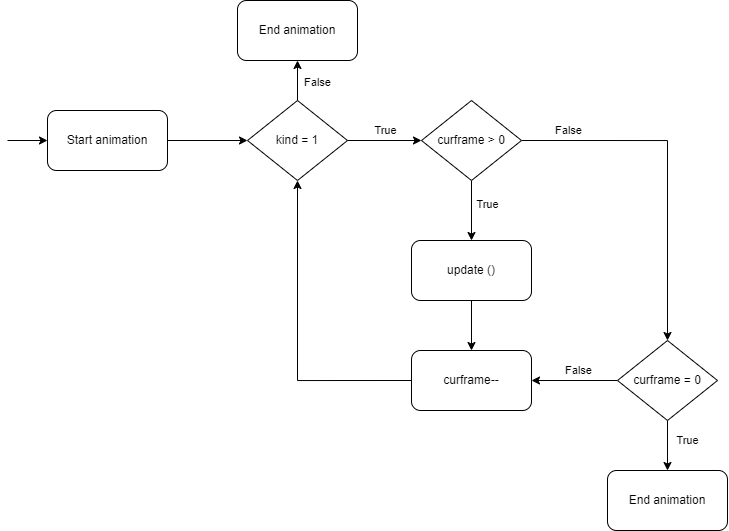
\includegraphics[scale=0.5]{img/exec.png}
        \caption{Graphe de flot de conrôle --- animation}
    \end{figure}
\end{center}

%Une fonctionnalité que j'ai pu implémenter pour le jeu et que j'ai trouvé intéressante est la caméra.
%Au début, nous avions un jeu avec un joueur que l'on pouvait déplacer mais lorsqu'on se déplaçait trop 
%d'un côté le joueur disparaissait. Il a donc fallu trouver un moyen de suivre le joueur dans le jeu.
%J'ai donc créé un objet caméra qui permettrait de voir le jeu non plus en partant de la position 0,0 
%mais à l'endroit où se trouve la caméra. Il a ensuite suffit de donner à la caméra la position du joueur 
%pour pouvoir suivre le joueur. Je vais expliquer dans cette section comment a été implémenté la caméra.

%Pour commencer la caméra a deux modes: \verb|position| qui place la caméra en fonction de son attribut 
%\verb|pos| et le mode \verb|player| qui place la caméra à la position du joueur. Ce second mode utilise 
%l'accès au joueur du fichier \verb|global.ml|. La vue est gérée dans le système \verb|view.ml|. Chaque 
%entité affichable (\textit{drawable}) possède un composant \textit{camera\_position} qui est la position 
%à l'écran. On différencie donc maintenant la position à l'écran et la position dans l'espace du jeu qui 
%est le composant \textit{position}. Le système \textit{view} va calculer à partir de la position de la 
%caméra et du composant la position à l'écran du composant. L'algorithme est plutôt simple, pour chaque 
%entité faire \verb|position_entité - position_caméra|. 

\subsection{Les ennemis (Ewen)}
Lorsque l'on a débuté la création des ennemis, nous avons commencé par créer un système \textbf{Ennemi} qui appelait 
une fonction \textit{pattern} à chaque frame et permettait ainsi de contrôler les comportements des ennemis. 
Nous avons commencé par essayer d'implémenter un composant qui simulait la vision d'un ennemi 
et se servait de l'algorithme de détection de collision. Pour ce faire, nous avions implémenté un nouveau composant 
\textit{vision} qui faisait apparaître un rectangle autour de l'ennemi mais ne corrigeait aucune collision. 
On pouvait alors détecter lorsque le joueur rentrait en collision avec la vision et ainsi appliquer un pattern à l'ennemi. 
Cependant, après divers tests et problèmes, nous avons décidé de garder la position courante du joueur dans 
une variable globale. Cela nous permet non seulement de réduire le nombre de composants, mais également d'appliquer plusieurs 
patterns différents selon la distance avec le joueur (cf. Alexandre le petit).
Par la suite, nous nous sommes rendu compte que nous pouvions utiliser le système \textbf{Real\_time} afin de contrôler 
le comportement des ennemis. Nous avons donc supprimé le système \textbf{Ennemi}.

Comme mentionné plus haut, il existe 3 types d'ennemis différents. Il y a tout d'abord les archers (composant \textit{arch})
 qui ne se déplacent pas et ne tirent que devant eux. 
Ils vérifient que le joueur se trouve bien à leur hauteur et à une certaine distance d'eux. Si les conditions sont vérifiées, 
ils tirent une flèche. Afin qu'ils ne tirent pas tout le temps, on utilise également une table de hachage qui stocke un cooldown. 
Ils ne tirent donc que si la condition sur le cooldown est vérifiée.

Ensuite, il y a les chevaliers (composant \textit{knight}). Ils commencent par 
vérifier que le joueur se trouve à une certaine distance d'eux. S'il est assez proche pour être vu, le chevalier va se rapprocher 
du joueur. Dès lors que le chevalier colle le joueur, il va mettre des coups d'épée afin d'infliger des dégâts.

Enfin, il y a le boss final, Alexandre le petit (composant \textit{Alexandre}). Tout comme les autres ennemis, 
il va commencer par regarder sa distance avec le joueur. Si le joueur est assez proche pour être vu, on prend 
la distance avec le joueur et on la fait passer à travers une fonction qui va donner un nombre entre 0 et 100. 
Ensuite, on tire au hasard un nombre entre 0 et 100, si il est plus grand que le premier nombre, on tire une boule de feu 
(on utilise également un cooldown). Si la distance est trop petite, le boss va se rapprocher du joueur jusqu'à 
ce qu'il soit à portée afin de l'attaquer au corps à corps.

Le boss étant un ennemi spécial et ayant beaucoup de vie, nous avons décidé d'implémenter une barre de vie qui 
apparaît en haut de l'écran. Cette barre est gérée par le composant \textit{hpbar}.

Enfin, comme il devient fréquent de prendre des dégâts, nous avons implémenté un composant de soin \textit{medkit}.
Il prend la forme d'un morceau de viande et lorsque que le joueur rentre en collision avec celui-ci, cela lui rend une 
partie de sa vie et le medkit est ensuite détruit.

\section{Les tests effectués}

Les tests du jeu se sont principalement fait avec la commande d'affichage en console afin de vérifier 
toutes les valeurs et intéractions entre les éléments du jeu. Les fichiers des niveaux ont également 
permis de simplifier le débogage avec la possibilité de mettre des commentaires. Ils permettent de 
facilement retirer un élément d'un niveau en le mettant en commentaire (sans pour autant tout supprimer).
Nous avons également développé divers outils permettant de tester notre jeu que nous allons maintenant 
présenter plus en détail. 

\subsection{Les hitbox}
Les hitbox sont les zones de collision des objets. Au départ, les collisions se faisaient en fonction de 
la taille des objets (un rectangle de 10x10 a pour collision l'ensemble de la zone de taille 10x10). Le 
problème avec cette méthode est que s'il y a une zone de transparence sur une texture, l'utilisateur voit 
une collision avec du vide. C'est la raison pour laquelle nous avons créé les hitbox. Une hitbox est 
simplement représentée par un décalage en x et en y et une taille w, h. Dans le système de collision on 
prend ensuite compte le décalage et la taille de la hitbox. Une hitbox n'est donc pas réellement une 
nouvelle box. Afin d'ajuster les hitbox au mieux nous avons donc créé un composant hitbox qui affiche 
la hitbox comme un rectangle au-dessus de l'entité. Ce premier outil nous a permis d'avoir des hitbox 
collisions réglées au pixel près.

\subsection{Le mode superuser}
Le mode superuser est un outil qui a été indispensable dans le développement du jeu. D'abord il permet 
d'accéder directement à un niveau en utilisant les touches 0 à 4, 0 étant le menu. Ensuite il permet 
également de modifier certaines constantes. Dans la configuration actuelle, on a par exemple les 
touches $u$ et $j$ pour augmenter et diminuer la vitesse du joueur.

Ce mode permet enfin de contrôler la caméra. La touche $p$ change le focus de \textit{player} à 
\textit{position}. En mode \textit{player} la caméra suit le joueur. En mode \textit{position} 
la caméra peut être déplacée. Le superuser permet de déplacer librement la caméra dans l'espace
 avec les touches \verb|oklm|. Cet outil a notamment été utile lors de la création des opnening 
 de niveau.

\end{document}